\documentclass{article}
\usepackage[utf8]{inputenc}
\usepackage{csvsimple,booktabs}
\usepackage{tabularx}
\usepackage{graphicx}
\usepackage{geometry}
\geometry{
	a4paper,
	total={170mm,257mm},
	left=20mm,
	top=20mm,
}
\title{Report of Analysis on BDjobs Data}
\author{SrJ}
\date{\today}

\begin{document}
	\maketitle
	
\section{Software Engineer}
\subsection{Analysis of Total Vacancy based on Top industries}
True in table \ref{tab:svac} means that there was significant difference in the job post during that time period.

In \textbf{Electronics / Consumers Durables} field there was a significant change in vacancy for software Engineer from 2016 to 2017 and 2017 to 2018. But Surprisingly there was no change from 2016 to 2018 i.e. in a two yr period. The explanation for this is the graph. From 16 to 17 in dropped abruptly and again from 17 to 18 it raised. So, on a two year run there was no significant difference but on one year run there was. Same pattern follows for Manufacturing Industries. See figure \ref{fig:svac} for details.

\begin{table}[!htb]
	\centering
	\caption{Analysis of Total Vacancy based on Top industries}
	\label{tab:svac}
	\csvautobooktabular{"Tables/Software Engineer_TotalVacancy_ttest.csv"}
\end{table}


\begin{figure}[!h]
	\centering
	\label{fig:svac}
	\caption{Total Numbers of Vacancy in Industry for \textbf{Software Engineer}}
	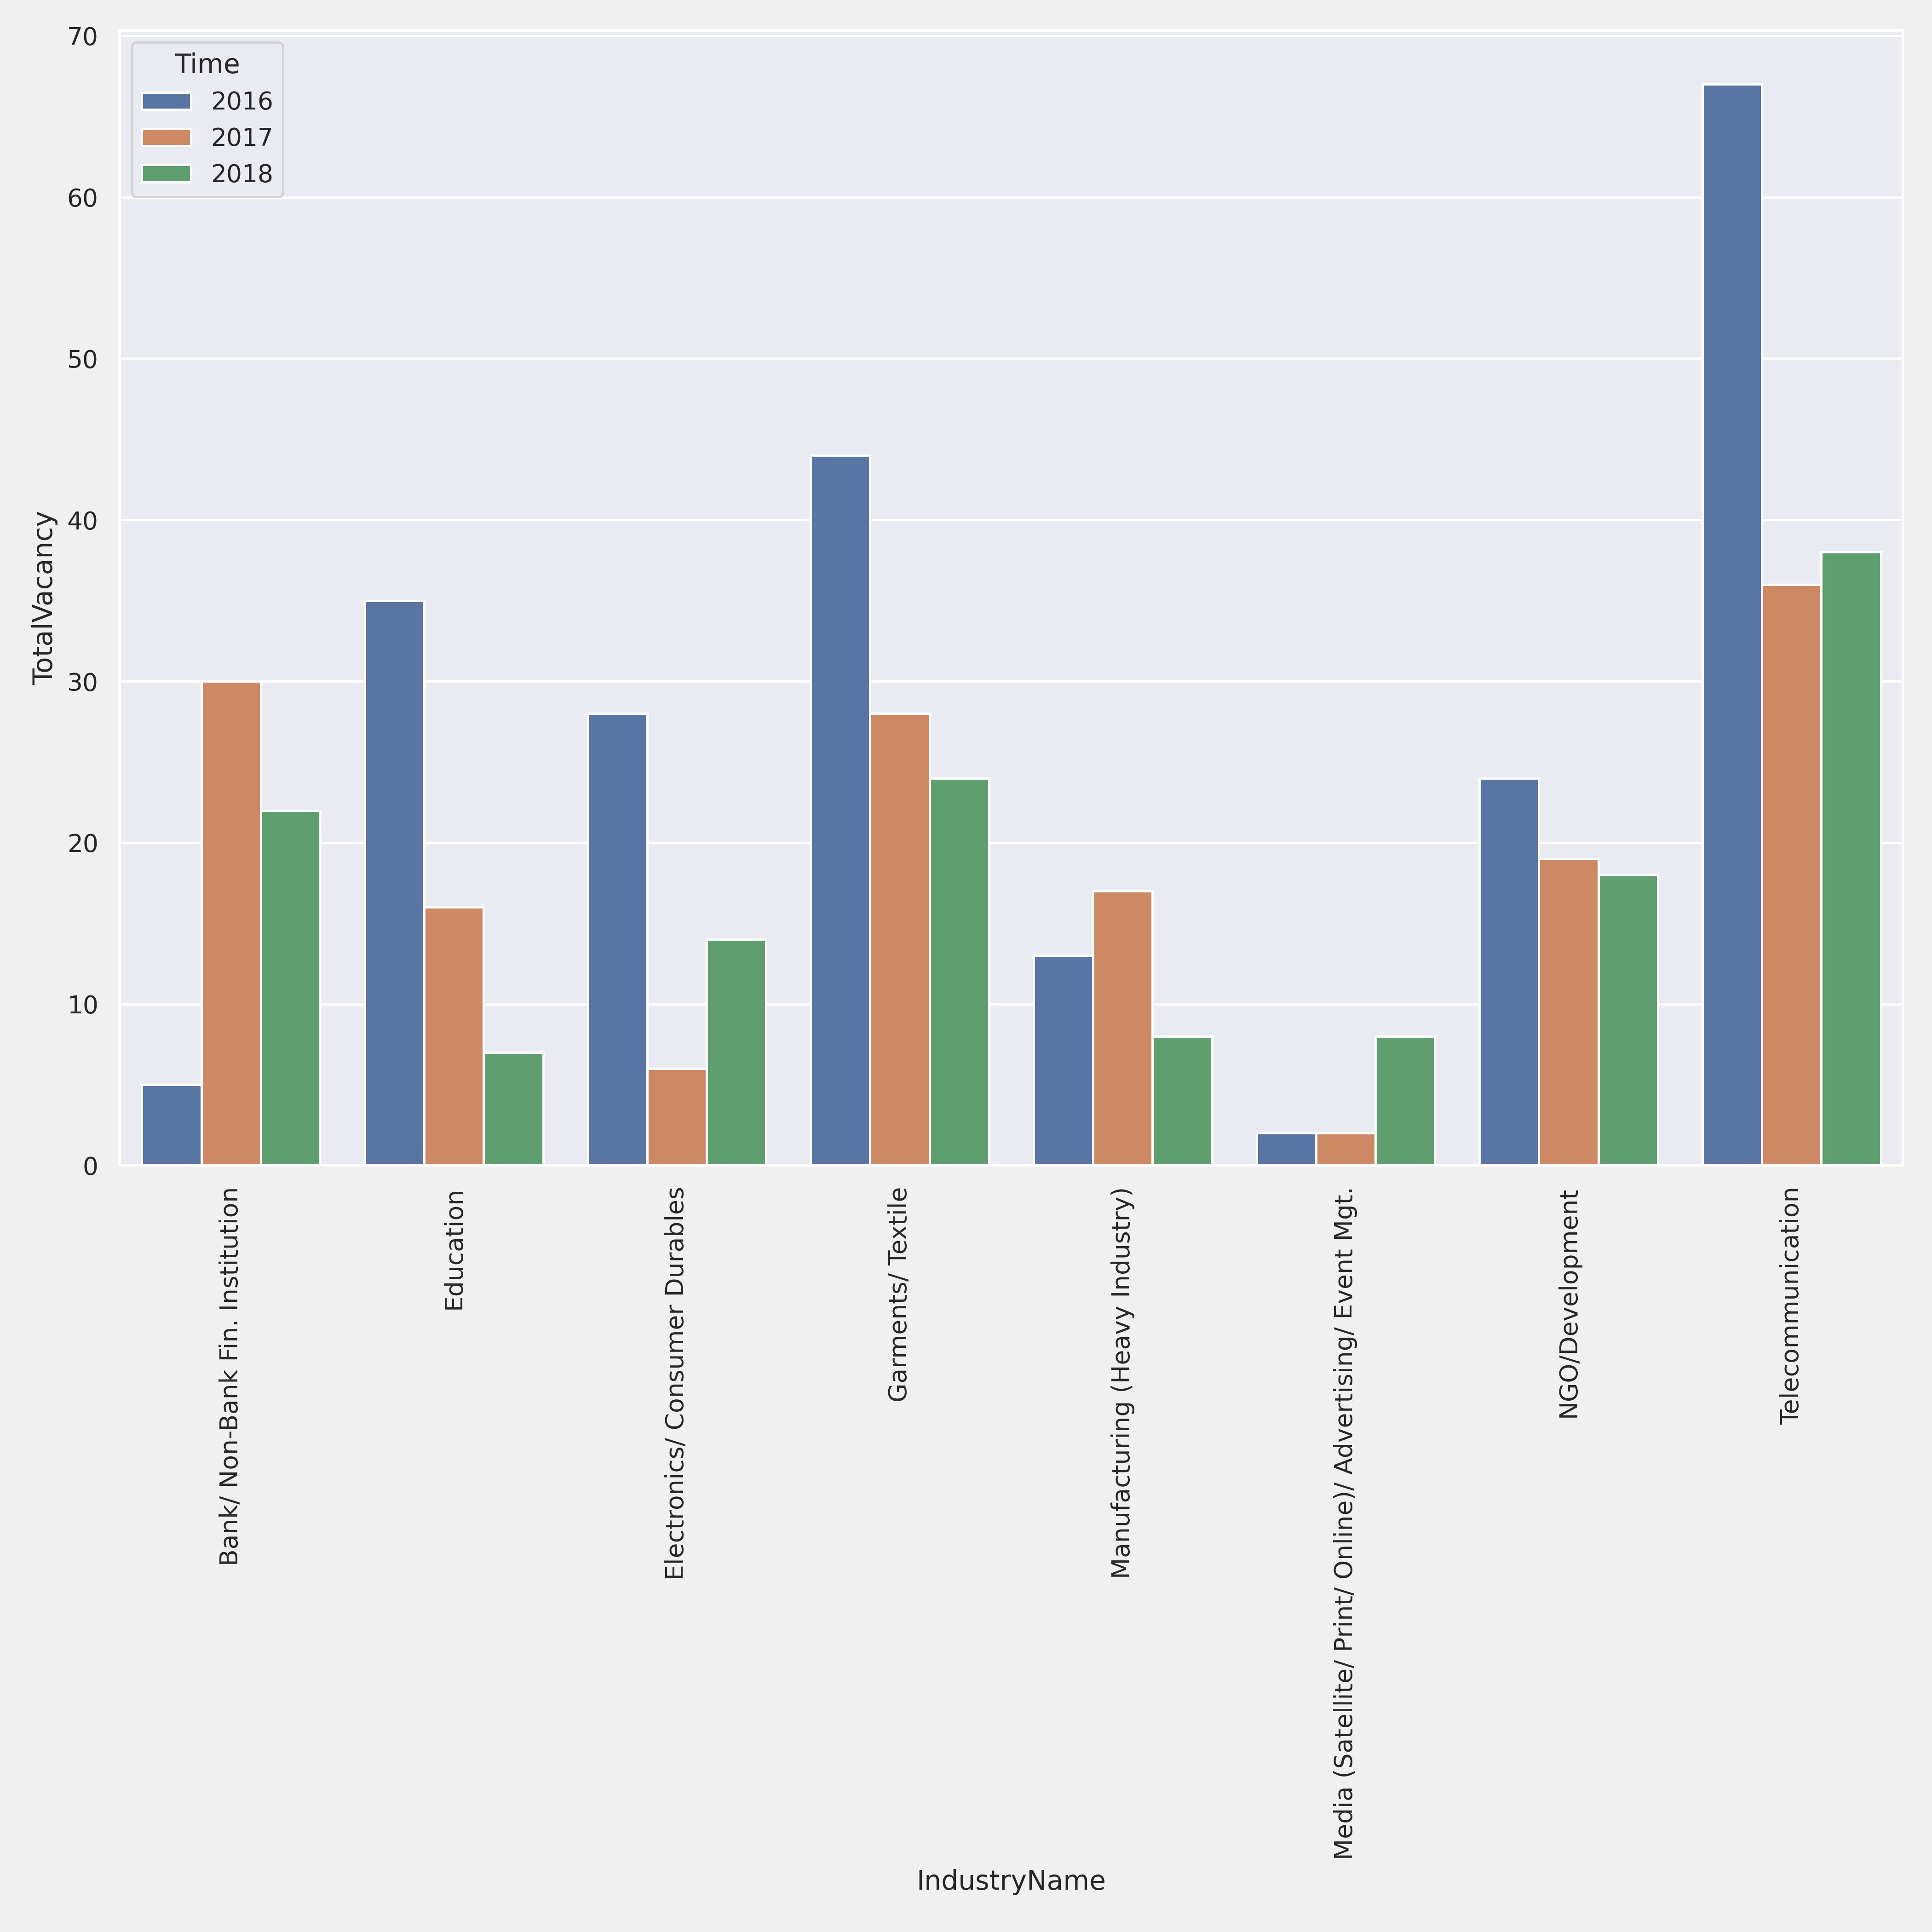
\includegraphics[scale=0.5]{Graphs/Software Engineer_TotalVacancy_ttest.png}
\end{figure}

\pagebreak
\subsection{Analysis of Total Applicant based on Top industries}
See figure \ref{fig:sapp} for details.

\begin{table}[!htb]
	\centering
	\caption{Analysis of Total Applicants based on Top industries}
	\label{tab:sapp}
	\csvautobooktabular{"Tables/Software Engineer_number_applicants_ttest.csv"}
\end{table}
\begin{figure}[!h]
	\centering
	\label{fig:sapp}
	\caption{Total Numbers of Applicants in Industry for \textbf{Software Engineer}}
	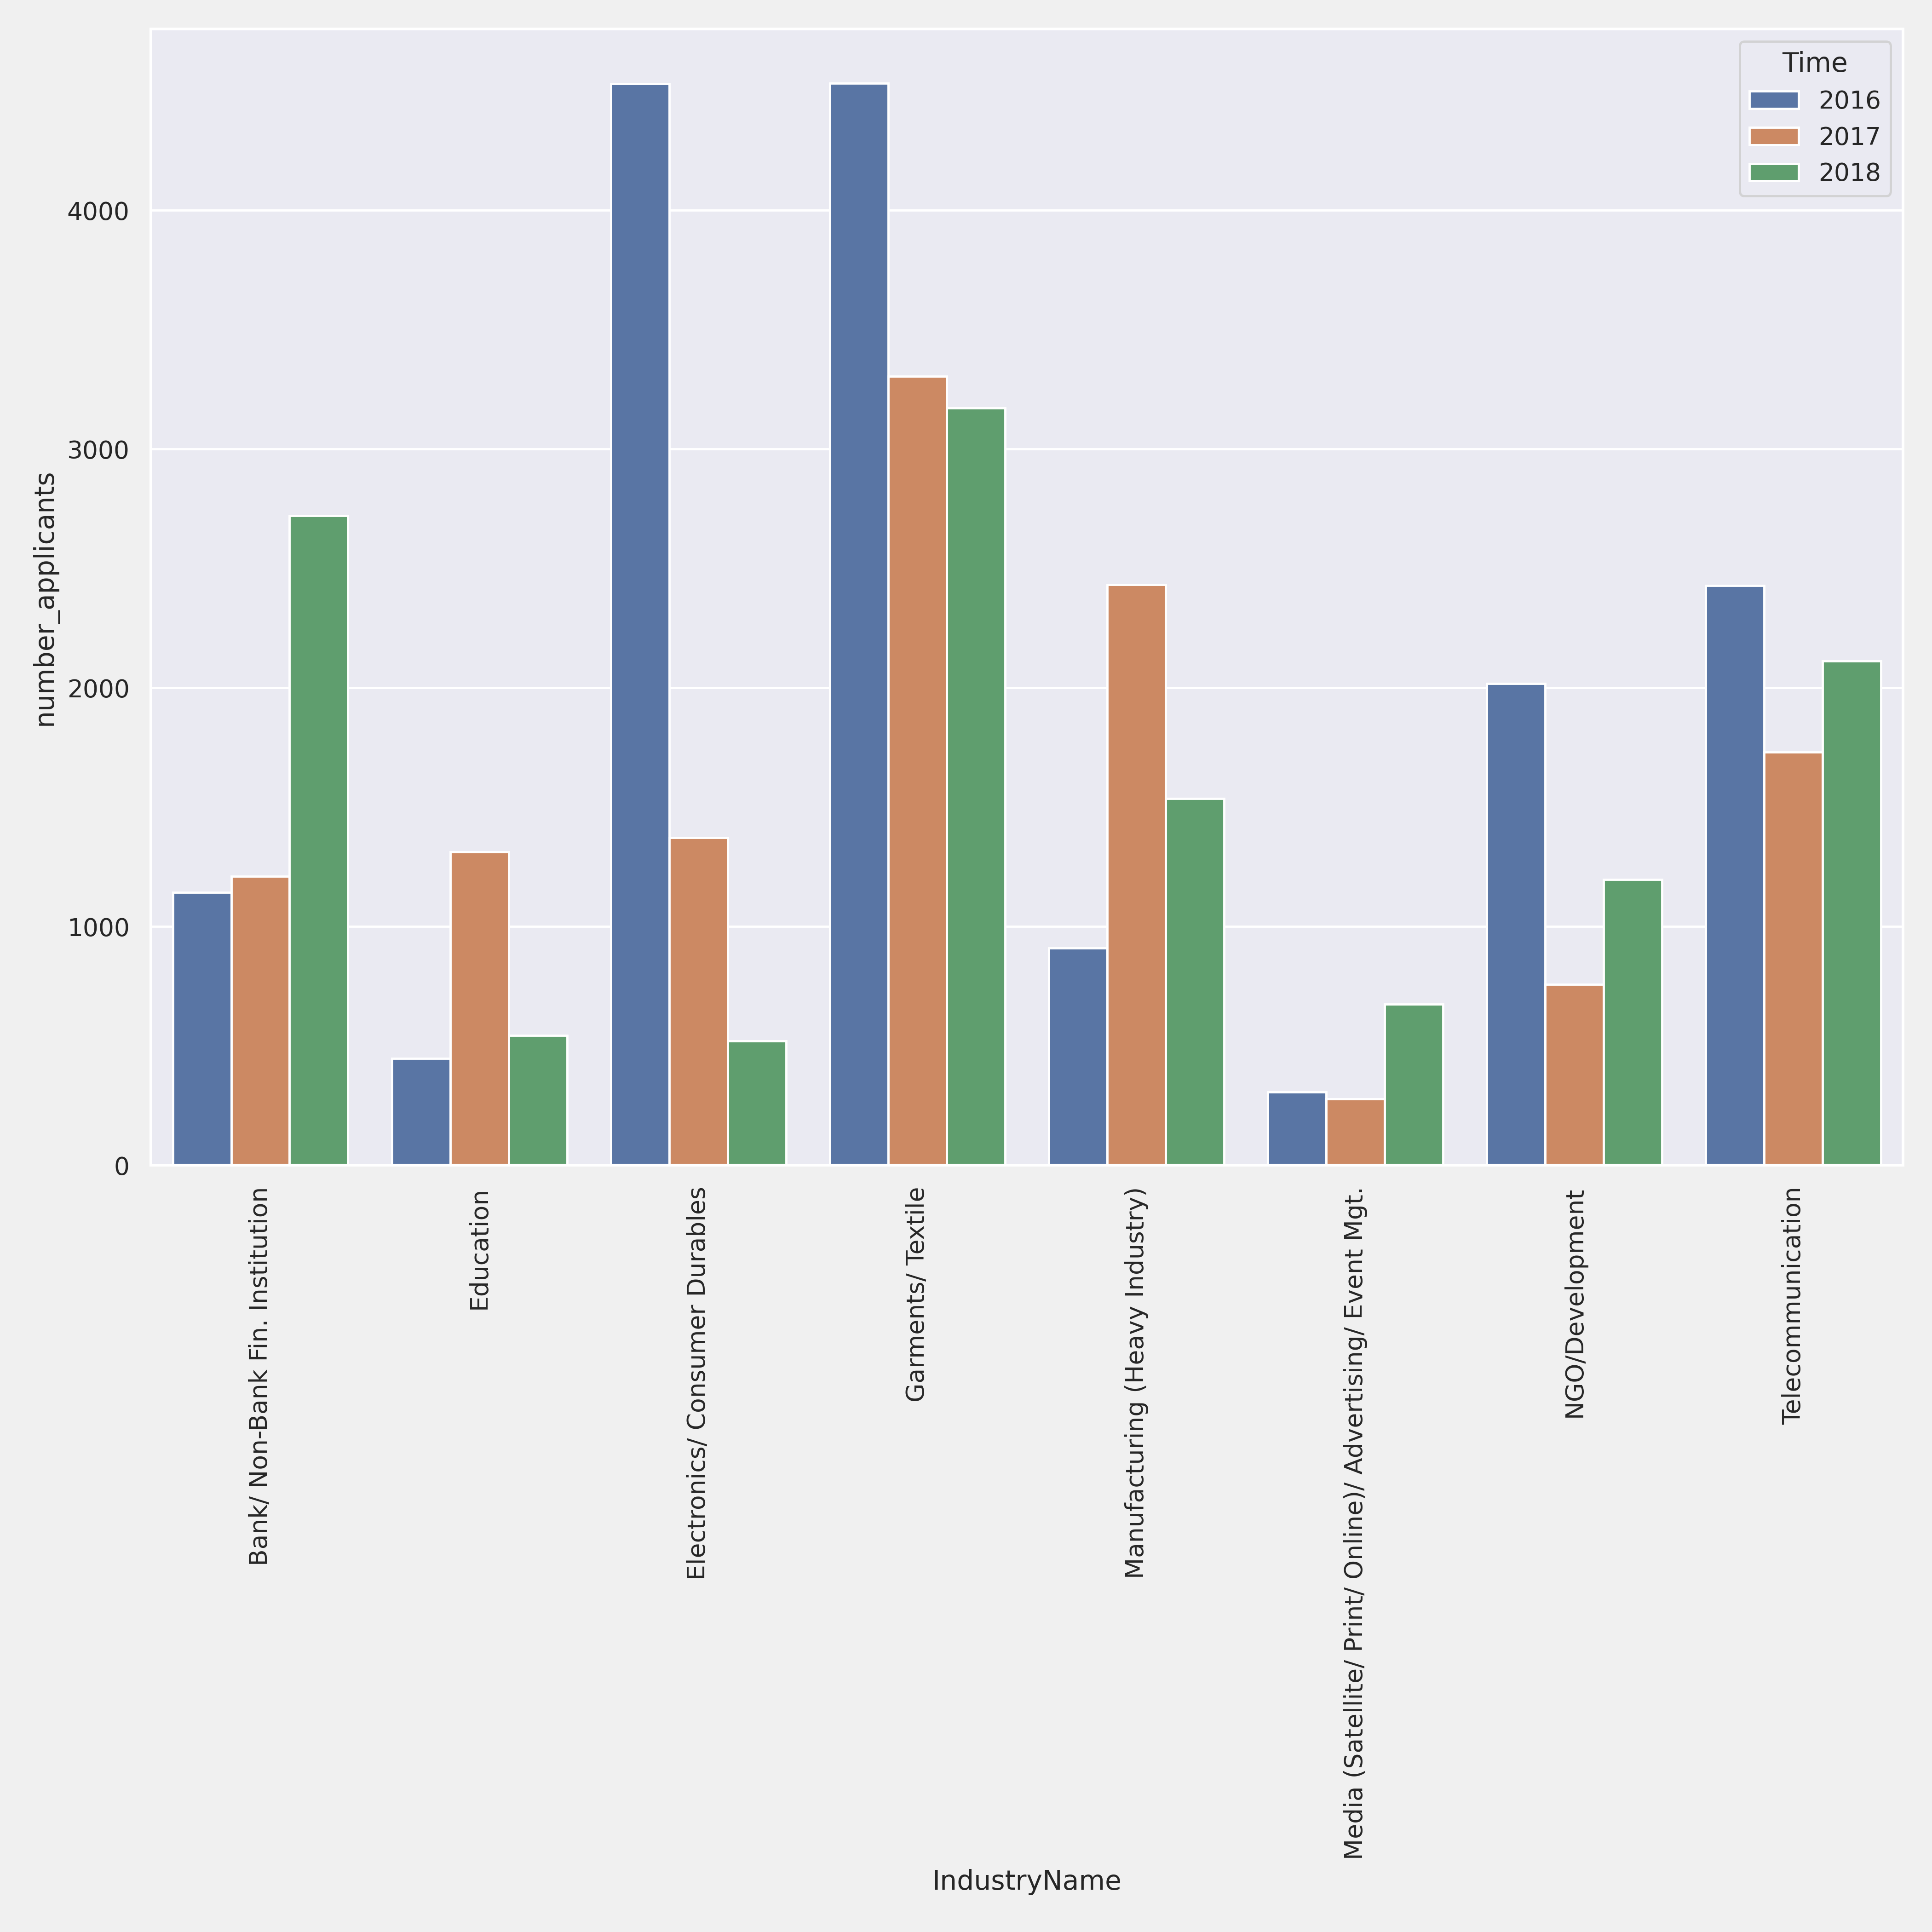
\includegraphics[scale=0.5]{Graphs/Software Engineer_number_applicants_ttest.png}
\end{figure}
\pagebreak

\section{Web Developer}
\subsection{Analysis of Total Vacancy based on Top industries}
True in table \ref{tab:wvac} means that there was significant difference in the job post during that time period.


\begin{table}[!htb]
	\centering
	\caption{Analysis of Total Vacancy based on Top industries}
	\label{tab:wvac}
	\csvautobooktabular{"Tables/Web Developer_TotalVacancy_ttest.csv"}
\end{table}


\begin{figure}[!h]
	\centering
	\label{fig:wvac}
	\caption{Total Numbers of Vacancy in Industry for \textbf{Software Engineer}}
	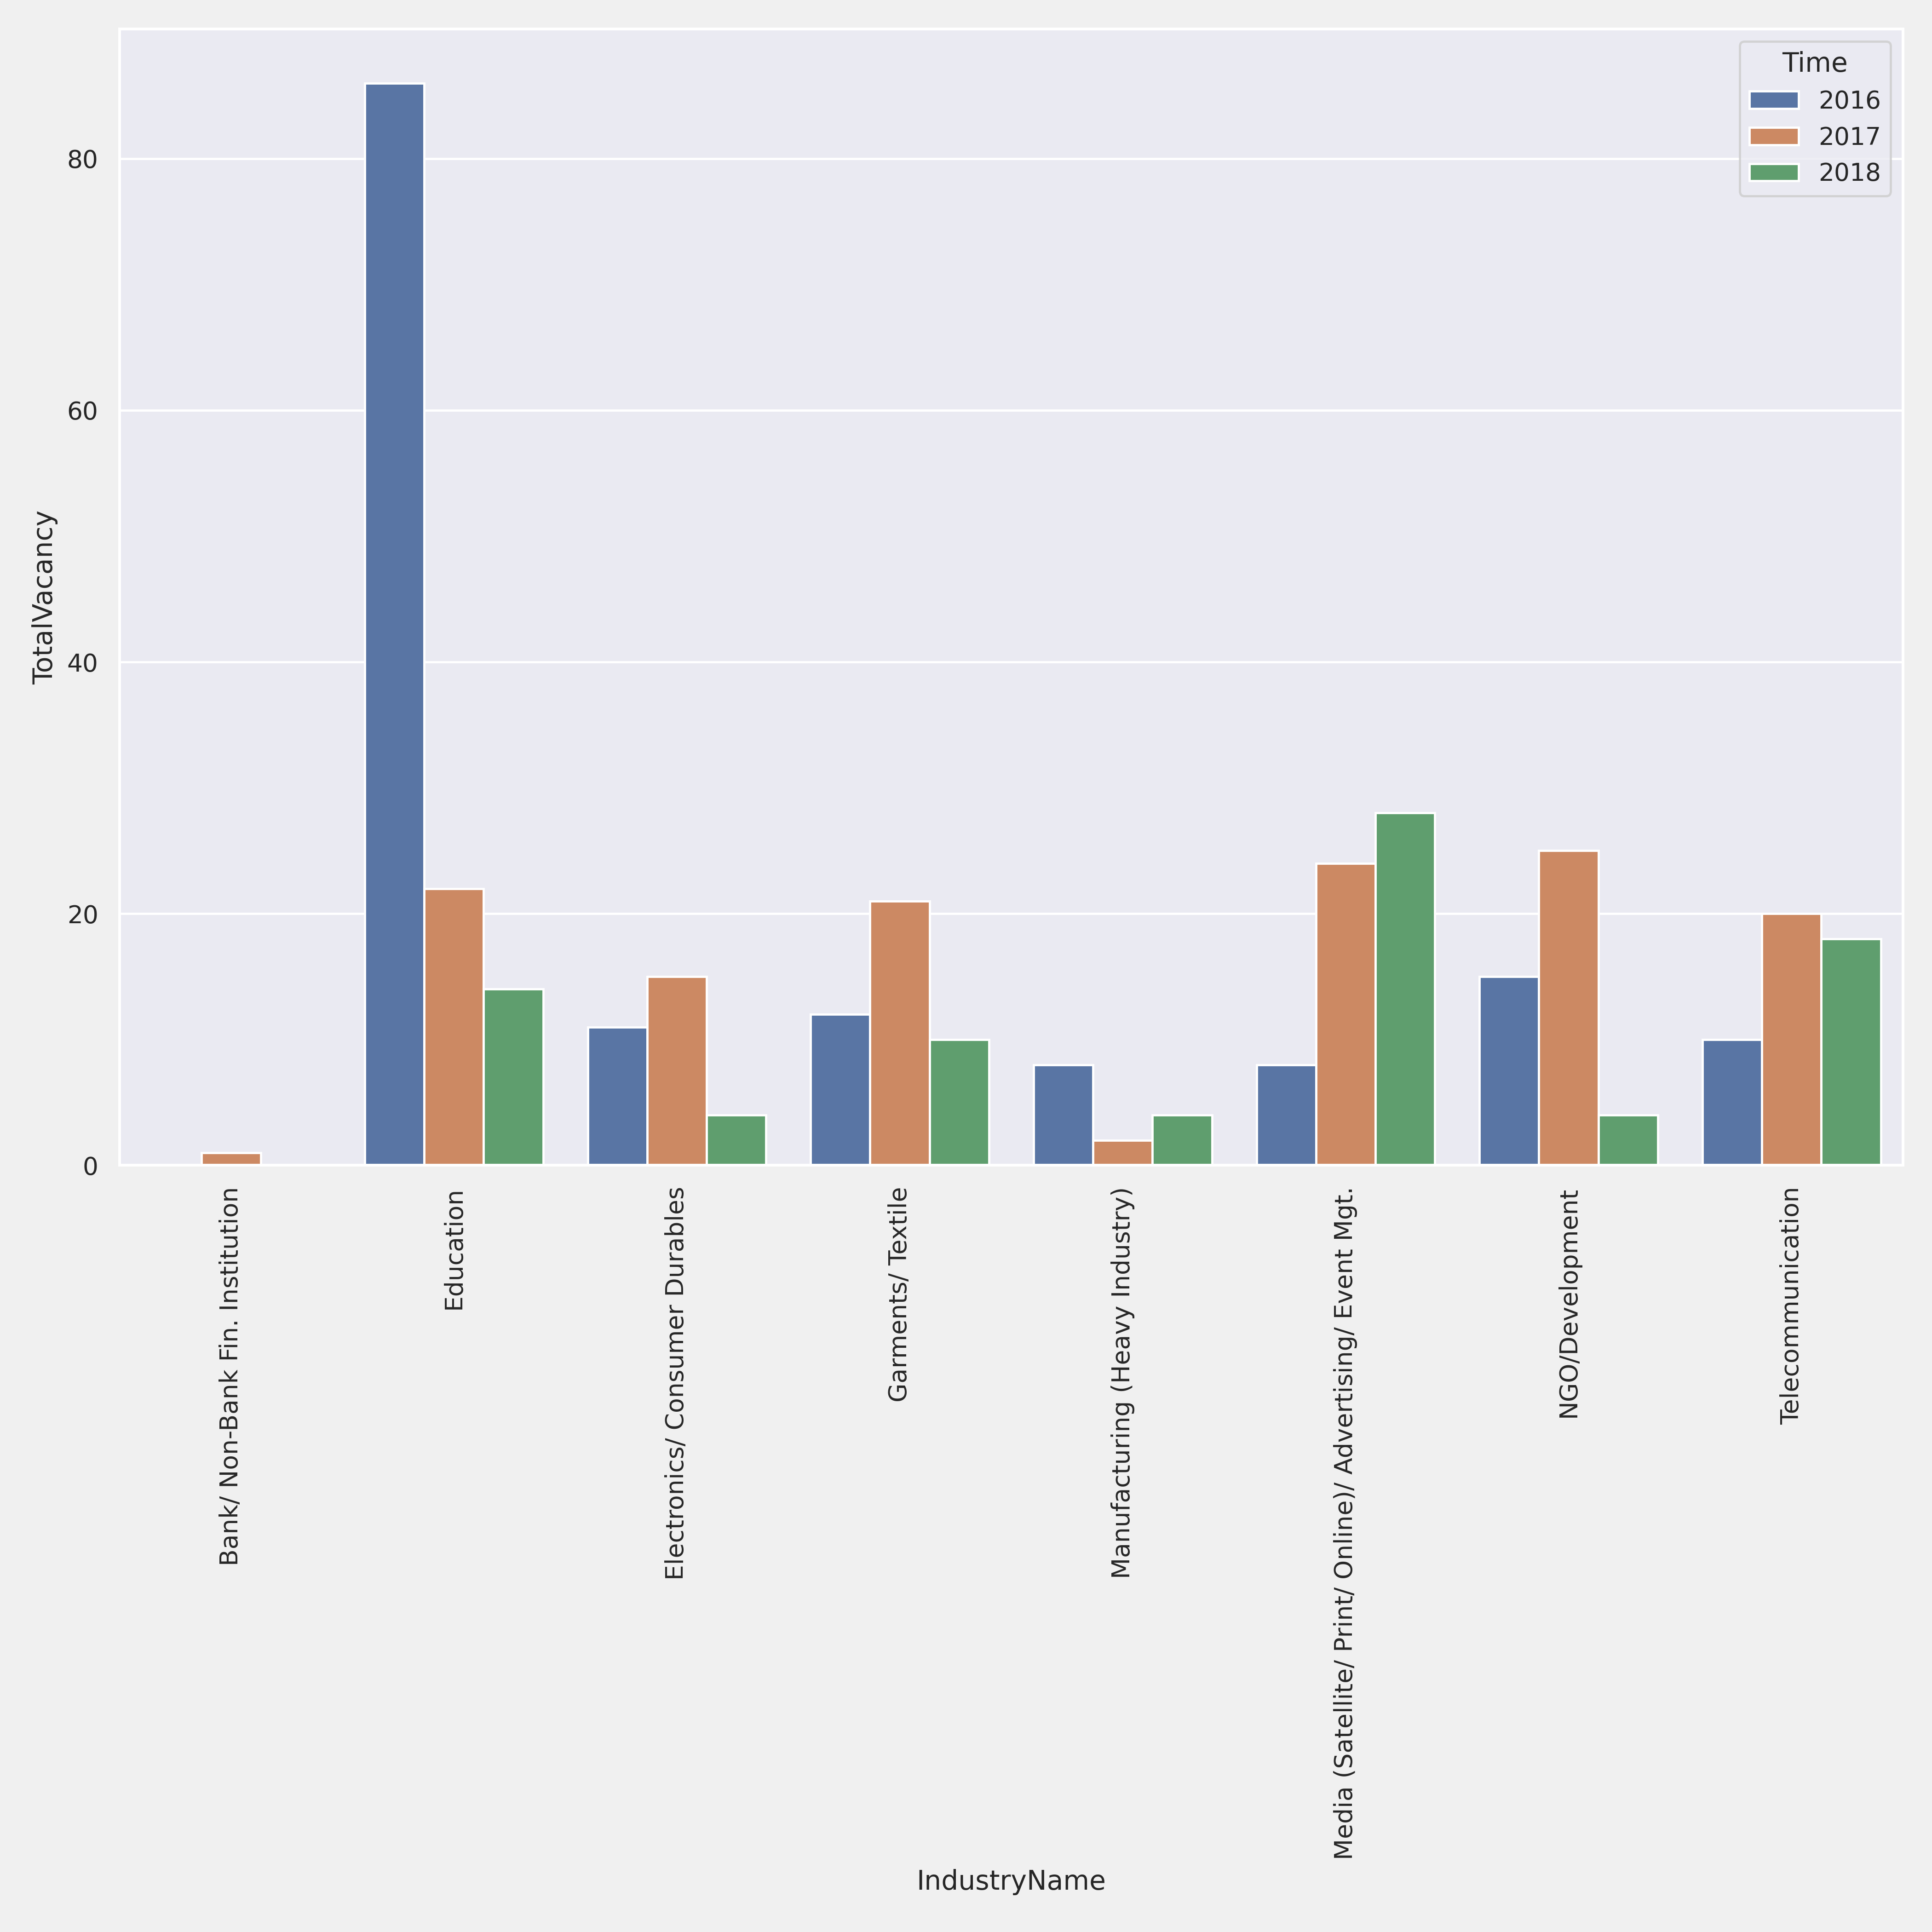
\includegraphics[scale=0.5]{Graphs/Web Developer_TotalVacancy_ttest.png}
\end{figure}

\pagebreak
\subsection{Analysis of Total Applicant based on Top industries}
See figure \ref{fig:wapp} for details.

\begin{table}[!htb]
	\centering
	\caption{Analysis of Total Applicants based on Top industries}
	\label{tab:wapp}
	\csvautobooktabular{"Tables/Web Developer_number_applicants_ttest.csv"}
\end{table}
\begin{figure}[!h]
	\centering
	\label{fig:wapp}
	\caption{Total Numbers of Applicants in Industry for \textbf{Software Engineer}}
	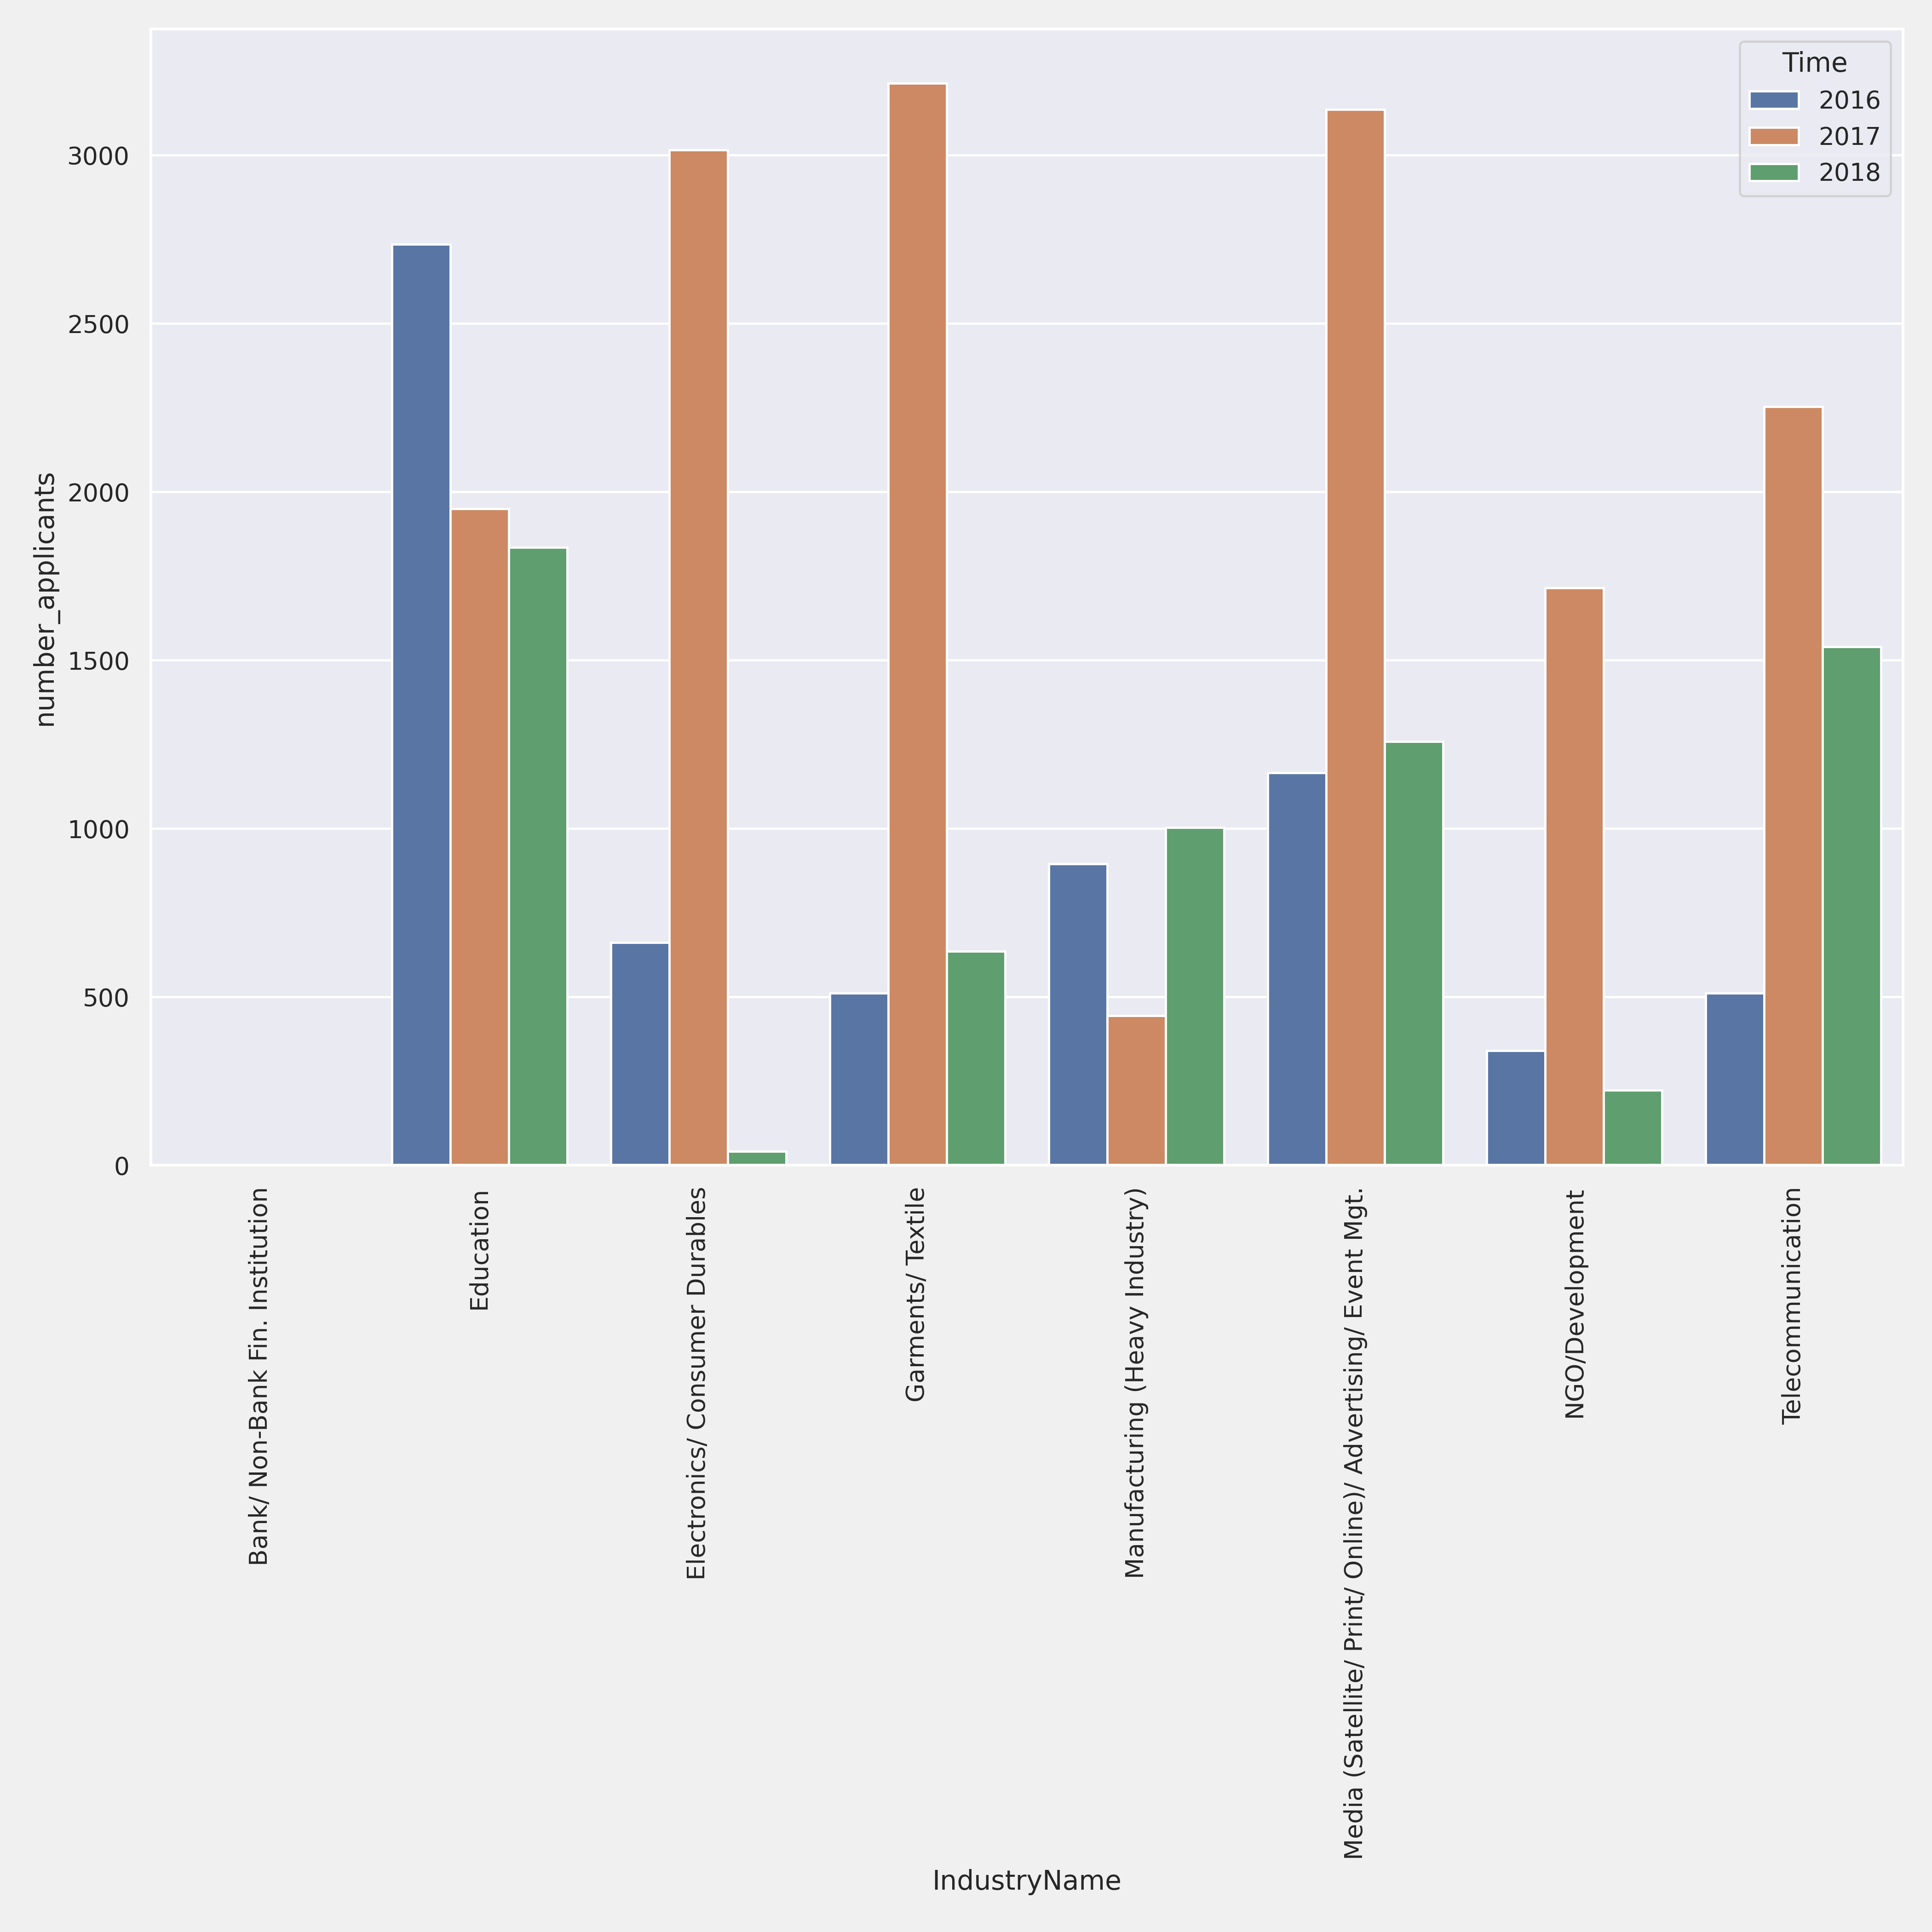
\includegraphics[scale=0.5]{Graphs/Web Developer_number_applicants_ttest.png}
\end{figure}

\end{document}